\chapter{Usage information}

The \OFEname \ application is available on Linux, Windows and MacOSX platforms.
We encourage you to use \OFEname \ program on Linux platform as it is the development and usually used platform. The following instructions mainly applies to Linux platforms.   

\section{Installation}

On linux platforms, the \OFEname \ software is available as distribution packages (deb, rpm) or archive files (tar.gz, tar.bz2).  
The recommanded way to install is to use packages for your Linux distribution. If you want to use archive files, you have to unarchive the software according to the directory tree.\\
Once installed, the \texttt{openfluid-engine} command should be available. You can check it by running the command \texttt{openfluid-engine} \verb?--?\texttt{help} or \texttt{openfluid-engine} \verb?--?\texttt{version} in your favorite terminal. You are now ready to run your first simulation.  

\section{Input dataset}

Before running the simulation, the input dataset must be built.
An \OFEname \ input dataset includes different informations, shared into many files:
\begin{itemize}
  \item the spatial domain definition
  \item the flux model definition
  \item the spatial domain input data 
  \item the discrete events
  \item the run configuration
  \item the outputs configuration
\end{itemize}

\noindent All these files must be placed into any directory that can be reached by the
engine. The default searched directory is a directory named
\texttt{.openfluid/engine/OPENFLUID.IN} and located into the user home
directory (the user home directory may vary, depending on the used operating
system). This directory is not automatically created, it should be created by hand.
If you prefer to place your dataset in another directory, you can
specify it using command line options passed to the engine (\texttt{-i} or \verb?--?\texttt{input-dir}).\\

\noindent In order to build these files, we encouraged you to use a good text editor, or better, an XML editor.
You can also use custom scripts or macros in specialized sotware, such as spreadsheets or Geographic Information Systems (GIS), to generate automatically the input dataset.

\bigskip

\section{Engine sequence}

The following sequence diagram describes the stage-by-stage execution of an \OFEname -engine simulation. The kernel is the main application, and the simulation function represents each simulation function used in the model definition.   

\begin{latexonly}
\begin{center}
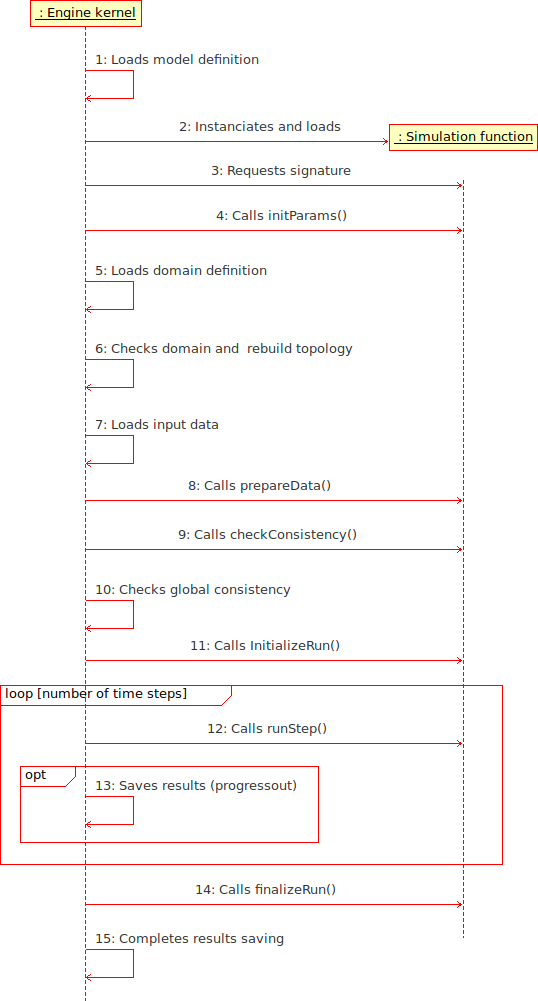
\includegraphics[scale=0.6]{common/graphics/ofeseq.png}
\end{center}
\end{latexonly}

\begin{htmlonly}
\begin{center}
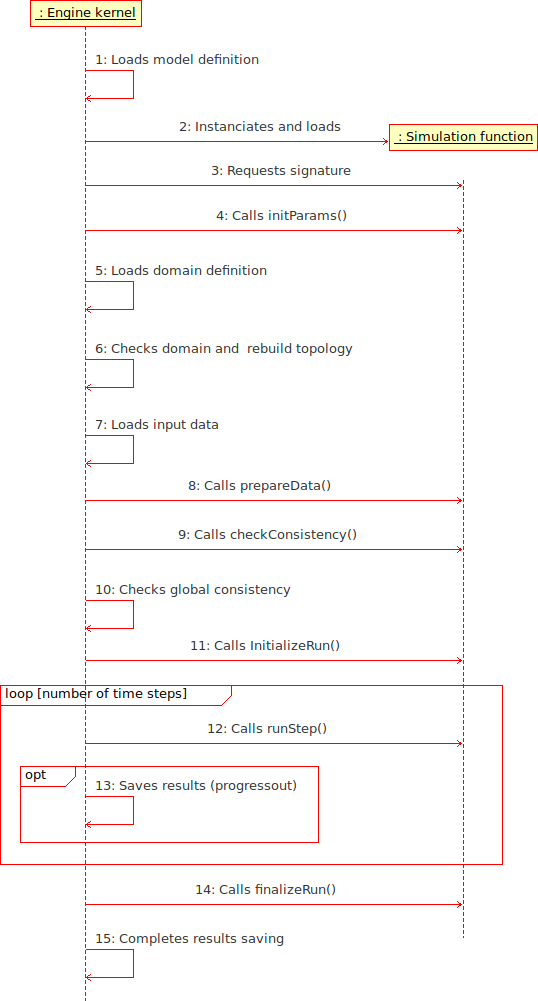
\includegraphics[scale=1]{common/graphics/ofeseq.png}
\end{center}
\end{htmlonly}

Stages description:
\begin{enumerate}
  \item the kernel loads the model definition (from the \texttt{model.xml} file)  
  \item the kernel loads and instanciates the simulation functions, according to the model definition
  \item the kernel requests the signature of each simulation function 
  \item the kernel runs the initParams() method of each simulation function
  \item the kernel loads the domain definition (from the \texttt{*.ddef.xml} files)
  \item the kernel check the domain definition consistency and rebuild the domain topology
  \item the kernel loads the domain input data (from the \texttt{*.ddata.xml} files)
  \item the kernel runs the prepareData() method of each simulation function
  \item the kernel runs the checkConsistency() method of each simulation function
  \item the kernel checks the global consistency (model + domain definition + domain input data)
  \item the kernel runs the initializeRun() method of each simulation function
  \item at every time step, the kernel runs the runStep() method of each simulation function
  \item at every time step, if the progressive output of results is enabled and if the current time step is a "progressive output time step", the kernel saves a packet of data and frees memory  
  \item the kernel runs the finalizeRun() method of each simulation function
  \item the kernel completes the save of results (all results if progressive output is disabled, the remaining results if progressive output is enabled) 
\end{enumerate}


\bigskip


\section{Run the simulation}

To run the simulation, if the dataset is located in the default searched directory, simply run the command \texttt{openfluid-engine} in your favorite terminal. 
To specify a different input dataset directory, use the \texttt{-i} or \verb?--?\texttt{input-dir} command line option.    

\bigskip

\begin{latexonly}
\begin{center}
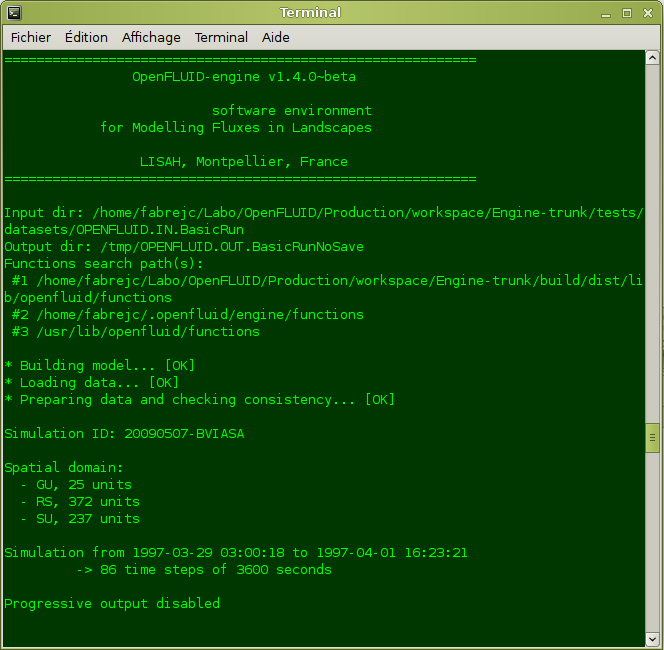
\includegraphics[scale=0.6]{common/graphics/oferun.png}
\end{center}
\end{latexonly}

\begin{htmlonly}
\begin{center}
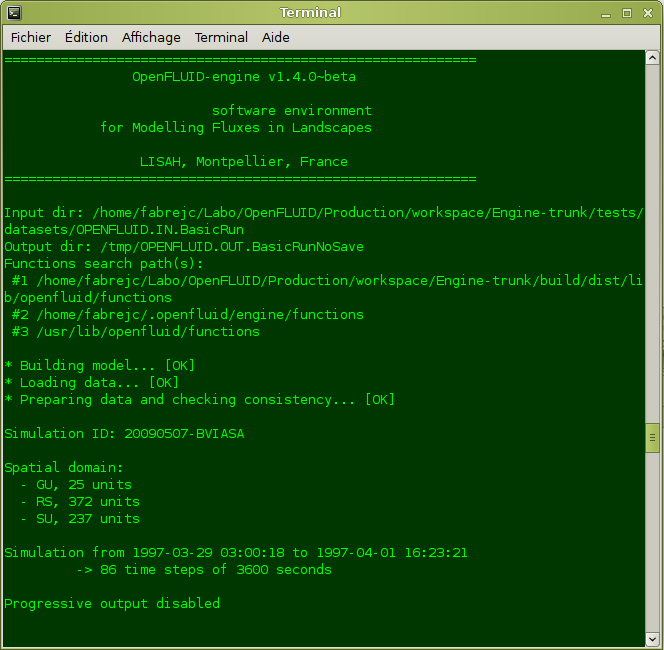
\includegraphics[scale=1]{common/graphics/oferun.png}
\end{center}
\end{htmlonly}

\section{Explore the results}

The results are stored in files, gathered by spatial unit. In each files, the values for variables are stored as columns, each row corresponfing to a data exchange time step (represented as a date and time).
The format of the files depends on the configuration of outputs, set through the \texttt{run.xml} file.
The default output directory is a directory named \texttt{.openfluid/engine/OPENFLUID.OUT} and located into the user home directory (the user home directory may vary, depending on the used operating system).
If you prefer to save your outputs in another directory, you can specify it using command line options passed to the engine (\texttt{-o} or \verb?--?\texttt{output-dir}).\\

\noindent In order to process the results of your simulations, we encourage you to use software environments such as R, Scilab or Octave, spreadsheets such as OpenOffice Calc, GIS such as GRASS or QGIS.   

\section{Buddies}

Buddies are small tools that help scientific developers in order to complete the modelling and/or development works. They are usable from the command line, using the \verb?--?\texttt{buddyhelp}, \verb?--?\texttt{buddy} and \verb?--?\texttt{buddyopts} options. Four buddies are available:
\begin{itemize}
  \item \texttt{func2doc}  
  \item \texttt{newfunc}
  \item \texttt{newdata}
  \item \texttt{convert}
\end{itemize}

\noindent Options are given to buddies through a comma-separated list of \texttt{key=value} arguments, using the \verb?--?\texttt{buddyopts} command line option.\\

\noindent General usage is:\\
\codeblock{openfluid-engine --buddy buddyname --buddyopts abuddyopt=avalue,
anotherbuddyopt=anothervalue}

\subsection{func2doc}

The \texttt{func2doc} buddy extracts scientific information from the source code of simulation functions. It uses the function signature and \LaTeX-formatted text placed between the \texttt{<func2doc>} and \texttt{</func2doc>} tags (usually into C++ comments). From these sources of information, it builds a \LaTeX\ document which could be compiled into a PDF document and/or HTML pages.\\
The \texttt{func2doc} buddy can also use information from an optional sub-directory named \texttt{doc}, located in the same directory as the input source file. The information in the \texttt{doc} subdirectory should be linked to the information from the source code using \LaTeX\ \texttt{\textbackslash input} command.  

\bigskip

\noindent Required options:
\begin{center}
\begin{tabularx}{\linewidth}{lX}
\texttt{inputcpp}&path for cpp file to parse\\
\texttt{outputdir}&path for generated files\\
\end{tabularx}
\end{center}

\noindent Other options:
\begin{center}
\begin{tabularx}{\linewidth}{lX}
\texttt{html}&set to 1 in order to generate documentation as HTML files\\
\texttt{pdf}&set to 1 in order to generate documentation as PDF file\\
\texttt{tplfile}&path to template file\\
\end{tabularx}
\end{center}

\bigskip

\noindent Usage example:\\
\codeblock{openfluid-engine --buddy func2doc --buddyopts inputcpp=/path/to/cppfile.cpp,
outputdir=/path/to/outputdir,pdf=1}


\subsection{newfunc}

The \texttt{newfunc} buddy generate a skeleton source code of a simulation function, using given options. 

\bigskip

\noindent Required options:
\begin{center}
\begin{tabularx}{\linewidth}{lX}
\texttt{cppclass}&C++ class name of the function\\
\texttt{funcid}&ID of the function\\
\end{tabularx}
\end{center}
    
\noindent Other options:
\begin{center}
\begin{tabularx}{\linewidth}{lX}
\texttt{authoremail}&email(s) of the author(s) of the function\\
\texttt{authorname}&name(s) of the author(s) of the function\\
\texttt{outputdir}&path for generated files\\
\end{tabularx}
\end{center}

\bigskip

\noindent Usage example:\\
\codeblock{openfluid-engine --buddy newfunc --buddyopts funcid=domain.subdomain.process.method,
outputdir=/path/to/outputdir}


\subsection{newdata}

The \texttt{newdata} buddy generate a skeleton dataset. 

\bigskip

\noindent Required options:
\begin{center}
\begin{tabularx}{\linewidth}{lX}
\texttt{outputdir}&Output directory for generated dataset\\
\end{tabularx}
\end{center}

\bigskip

\noindent Usage example:\\
\codeblock{openfluid-engine --buddy newdata --buddyopts outputdir=/path/to/outputdir}

\subsection{convert}

The \texttt{convert} buddy converts a dataset from a specific version format to another one. Currently, conversion is only possible from 1.3.x format to 1.4.x format. 

\bigskip

\noindent Required options:
\begin{center}
\begin{tabularx}{\linewidth}{lX} 
\texttt{convmode}&Conversion mode. Available modes are: \texttt{13\_14}\\
\texttt{inputdir}&Input directory for dataset to convert\\ 
\texttt{outputdir}&Output directory for converted dataset\\
\end{tabularx}
\end{center}

\bigskip

\noindent Usage example:\\
\codeblock{openfluid-engine --buddy convert --buddyopts convmode=13\_14,
inputdir=/path/to/inputdir,outputdir=/path/to/outputdir}


